\documentclass[a4paper,14pt]{extreport}

% packages to support Cyrillic fonts, needed to write abstracts
\usepackage[T2A]{fontenc} 
\usepackage[utf8]{inputenc} 
\usepackage[russian,english]{babel}
\usepackage{csquotes}

% usual packages
\usepackage[left=30mm, right=10mm, top=20mm, bottom=20mm]{geometry}

\usepackage{graphicx} % to add figures
\graphicspath{{figures/}}

\usepackage{hyperref} % to add clickable contents menu

\usepackage[ natbib=true, style=numeric,sorting=none]{biblatex}
\addbibresource{bibliography.bib}

\usepackage{blindtext}

% the following three definitions are to be changed by student
\def\myauthor{Aldabergenova Dana\\Namazbayev Almas\\Oralova Zhanel\\Baimolda Aray\\Bolatbek Gaukhar} % author
\def\mycoach{Ardak shalkarbay-uly} % coach, adviser etc.
\def\mytitle{Trading platform for a used goods store with the possibility of selling vintage goods and organizing auctions.} % title
\def\mydegree{Bachelor in Computer Systems and Software}
\def\mydegreecode{5B070400}
%\def\mydegree{Bachelor in Сomputer Science}
%\def\mydegreecode{6B06102}

% preamble ends here

\begin{document}
    % don't touch these two lines :)
    \begin{titlepage}
\begin{center}
\large
Ministry of Education and Science of the Republic of Kazakhstan

Suleyman Demirel University

\vspace{1cm}
\begin{figure}[h]
    \centering
    
\includegraphics[scale=0.5]{sdu_only}
\end{figure}

\vspace{2cm}
\Large
\myauthor

\vspace{1cm}
\Large
\textbf{\mytitle}

\vspace{1cm}
\large
A thesis submitted for the degree of

\mydegree

(degree code: \mydegreecode)

\vfill
Kaskelen, 2022

\end{center}
\end{titlepage}
    \newpage
\pagestyle{empty}

\begin{center}
\large
Ministry of Education and Science of the Republic of Kazakhstan

Suleyman Demirel University

Faculty of Engineering and Natural Sciences

\vspace{2cm}
\textbf{\mytitle}

\vspace{1cm}
\large
A thesis submitted for the degree of

\mydegree

(degree code: \mydegreecode)

\vspace{2cm}
Author: \textbf{\myauthor}

\vspace{2cm}
Supervisor: \textbf{\mycoach}

\vspace{2cm}
Dean of the faculty:

\textbf{Assist. Prof. Azamat Zhamanov}


\vfill
Kaskelen, 2022
\end{center}
    
    % edit abstracts
    \newpage
\pagestyle{plain}

{\selectlanguage{english}
\begin{center}
    \Large
    \textbf{Abstract}
\end{center}
The fashion industry is one of the industries that pollute the environment and is in second place in terms of consumption after water. At the moment, many people are striving for a more environmentally friendly approach to clothing and second-hand stores are a good solution. Also, the concept of second-hand and "vintage" clothing is gaining popularity among the young generation, as it allows you to purchase unique items at an affordable price. In Kazakhstan, this activity is carried out through social networks and there is no integrated online platform with online processes, which complicates the search and purchase of things for buyers and sellers. For this reason, we want to demonstrate an alternative for stores, a trading platform with the ability to put unique items up for auction.
}
    \newpage
\pagestyle{plain}

{\selectlanguage{russian}
\begin{center}
    \Large
    \textbf{Аңдатпа}
\end{center}
Головкиннің әуесқой мансабы ұзаққа созылды әрі қанық, оқиғаға толы болды. Генадий бокспен 8 жасынан бастап айналыса бастады. 1993 жылы оны облыстық бокстан өткен жарысқа оның бапкері жіберген болатын. Соңында осы сайыстан 3 жеңіс әкелді. Бұдан кейін ол облыстық, мемлекеттік және халықаралық бокстан жарыстарға үміткер болып қатыса бастады. Осы уақытқа дейін Генадий Головкин өзінің қатысқан 350 жекпе-жегінде тек 5 рет қана жеңіліске ұшыраған болатын.19 жасында шығыс боксында бірінші орын алады да, 2002 жылы бұл жеңісін тағы бір мәрте қайталайды. 2003 жылы Таиландта өткен боксшылар жекпе-жегінде өзінің 4 қарсыласының екеуін нокаутқа жібергені үшін бірінші орынды алады.
}
    \newpage
\pagestyle{plain}

{\selectlanguage{russian}
\begin{center}
    \Large
    \textbf{Аннотация}
\end{center}
Индустрия моды является одной из отраслей, загрязняющих окружающую среду и находится на втором месте по потреблению после воды. На данный момент многие люди стремятся к более экологичному подходу к одежде и хорошим решением служат секонд хенд магазины. Также, концепция секонд хенда и «винтажной» одежды набирает популярность среди молодого поколения, так как позволяет приобретать уникальные вещи по доступной цене. В Казахстане эта деятельность осуществляется через соц. сети и нет объединенной онлайн площадки с онлайн процессами, что усложняет поиск и покупку вещей для покупателей и продавцов. По этой причине, мы хотим продемонстрировать альтернативу для магазинов, торговую платформу с возможностью ставить уникальные вещи на аукцион.  

}
    \tableofcontents
    
    % edit your chapters
    \chapter{Introduction}\label{ch:intro}
%these sections are optional, up-to the author
\section{Motivation}
\section{Aims and Objectives}
\section{Thesis Outline}
The first chapter is \nameref{ch:intro} chapter. It is this one that you are currently reading. It gives insight into the work done. In Chapter \ref{ch:A} we review related work and formulate the problem to solve. Chapter \ref{ch:B} is describing the solution to the problem. And in \nameref{ch:concl} chapter we conclude our conclusion.
    \chapter{Project details}\label{ch:A}
\section{Research}
Before starting the project, we consulted with many people. Since it isn't a simple process to create a web application. After that, we came to the decision to do detailed analysis of our next steps of the project. For that, we divided into several steps:
    
    1. What is our project and its main purpose and what target audience will use the application
    
    2. What features will there be 

    3. What will we have to do to achieve our goals

    4. What technologies will be used

Through the research, we found out the approximate number of people who are interested in this area and approximately how many people will use our application. Because of this, we began to understand how to move on. We took note of what problems might be in the future and began to understand how to implement our project.

The next phase of the project is market analysis. Where each of us should explore other alternatives and describe exactly how their system works, the pros and cons, as well as the errors of the services.

Further, due to the analysis, we decided to make a web-site. Where access will be for all users, regardless of the operating system of the device.

And finally, our goal is to make a good product that will be useful for people. As we said earlier, second-hand shops are very useful for the environment and we hope that our project will be useful for people and it will become more convenient for them to purchase things. Our team aims to develop this project further and will add new features in future.

%Let us cite some resources form the  bibliography. This is a a good book \cite{dirac}. Let's cite Einstein's paper \cite{einstein} and Knuth's website \cite{knuthwebsite}. Knuth has also a book on algorithms \cite{knuth-fa}.%
\section{Pain points and importance of the project}
Initially, when our team was on process of discussion of the project and the main theme. The first pain point was auction-system.

Since there is no such platform in Kazakhstan, it was not entirely clear how to implement the auction and store system at the same time. 
The solution to this problem was foreign alternative websites. More specifically, eBay.
Where the seller enters the initial amount of money and sets the period for which this lot can be bid.

The second pain point. Our problem was to find people who had experience with vintage items, as the second hand in Kazakhstan are not so popular. But we solved this problem in the following way, we started writing to people who were subscribed to the account of vintage stores. Many of them agreed to take the survey, which helped to understand the market situation. And also communicate with some buyers, and found out that the demand for vintage items increased from year to year. Thanks to the survey, we found out that most people are not comfortable looking for things in a standard way, as it takes them a lot of time and effort, but this also applies to store owners. Our main goal is to improve this process by creating a platform that automates this process without changing the fundamental business logic.

\section{Planning and defining risks}
Since every project has its own problems, we decide what method our team should choose, so that our team can quickly sort out the problems. 

We needed a method which would help our team work together. Our team was thinking about the most convenient method and also not too hard to work with, since we are just starting our journey in the IT sphere.  

Before starting the project, we thought for a long time about which management method is most suitable. Our choice fell into the scrum method.

There are many methods like Agile, Kanban, etc. But for us the most effective was scrum. 
Scrum is a setting of meeting, planning and tools in a team, that helps to better manage the work in teamwork. 
Scrum - allows us to adapt to constantly changing conditions of the project.
This method has its own artifacts or also called tools.  
Scrum have 3 solving tools:

-Backlog of project

-Backlog of sprint

-Increment. 

As for the juniors, it was the best method for us. 
Our team had everyday short calls, where every member of the team discussed their progression. And if someone had problems or some misunderstanding, they 
discussed it with the project manager. 

We look forward to implementing more new features in our platform and hope that our project will continue to grow. 




    \chapter{Project Architecture}\label{ch:B}

\section{Hierarchy}
Since we have few roles in the web-site. We would like to show you hierarchy of users. (See Figure \ref{fig:Hierarchy}).

\begin{figure}[h!]
    \centering
    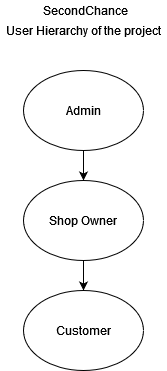
\includegraphics[scale=0.9]{figures/Hierarchy.png}
    \caption{User types}
    \label{fig:Hierarchy}
\end{figure}

\section{User case diagram}
This is a use case diagram, where you can understand how all system users work
In our case, there are three roles - Admin, Shop Owner, Customer.  Each of them has their own individual roles that are interconnected.  The admin can add or remove shop owners and stores.  And in turn, Shop Owners create or delete a store product, and they can also edit products.  For example, they can change the time of the auction.
Customers can purchase items only after registration. (See Figure \ref{fig:user-case}).

\begin{figure}[h!]
    \centering
    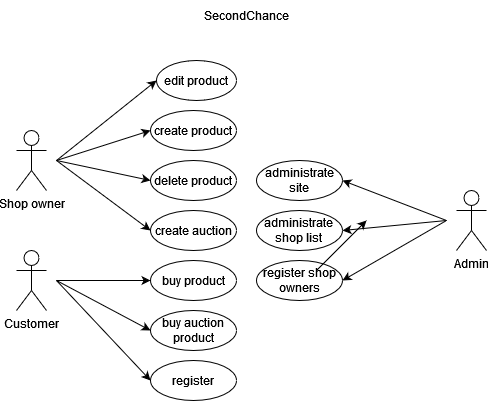
\includegraphics[scale=0.9]{figures/user-case.png}
    \caption{User-case diagram}
    \label{fig:user-case}
\end{figure}
\clearpage


\section{Activity diagram}
The activity diagram describes the actions that are performed on the web-site. Clients should have a registered account to purchase the product. If the client does not have it, he would not be able to buy selected products. Next step is checking if the product is still available or not. If not, the actions will end. When a selected product is available, the next action is payment. Only on condition that the payment goes through, the order is confirmed. If payment does not go through, the process ends without purchasing the product. (See Figure \ref{fig:activity-shop}).

\begin{figure}[h!]
    \centering
    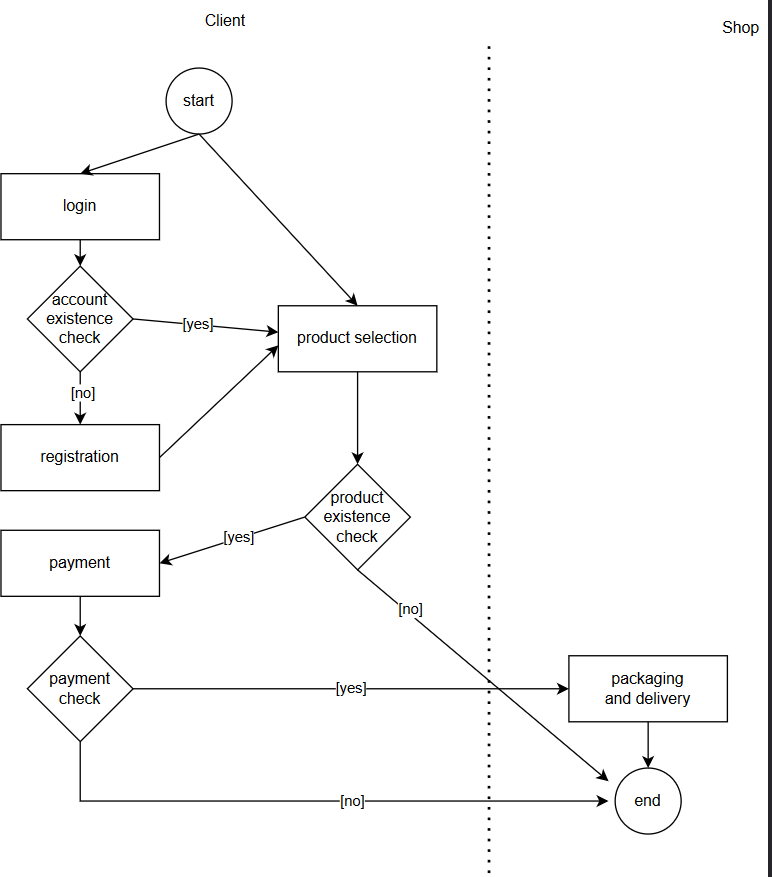
\includegraphics[scale=0.6]{figures/activity-shop.png}
    \caption{Activity-shop diagram}
    \label{fig:activity-shop}
\end{figure}
\clearpage

The last diagram was about the shop system. This one shows the functionality of the auction system. (See Figure \ref{fig:activity-auction}).

\begin{figure}[h!]
    \centering
    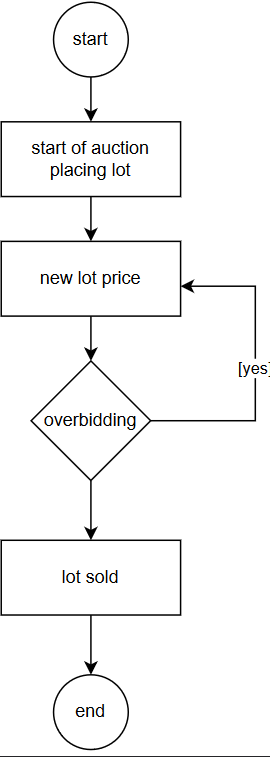
\includegraphics[scale=0.6]{figures/activity-auction.png}
    \caption{Activity-auction diagram}
    \label{fig:activity-auction}
\end{figure}


    \chapter{Implementation}\label{ch:C}
\section{Design process}
UX/UI design is one of the earliest and the most important stages of building a successful project. To make it more conscious and consistent, we started from market and user researches using methods such as survey, analysis of analogues, user stories and user personas. The goal was to answer questions:

- What problem do your users need solving?

- What are their behaviors, needs and motivations?
Finally on this stage, we formed two user personas that approximately describe future ordinary users of the website. (See Figure \ref{fig:image001}, \ref{fig:image003}).
\begin{figure}[h]
    \centering
    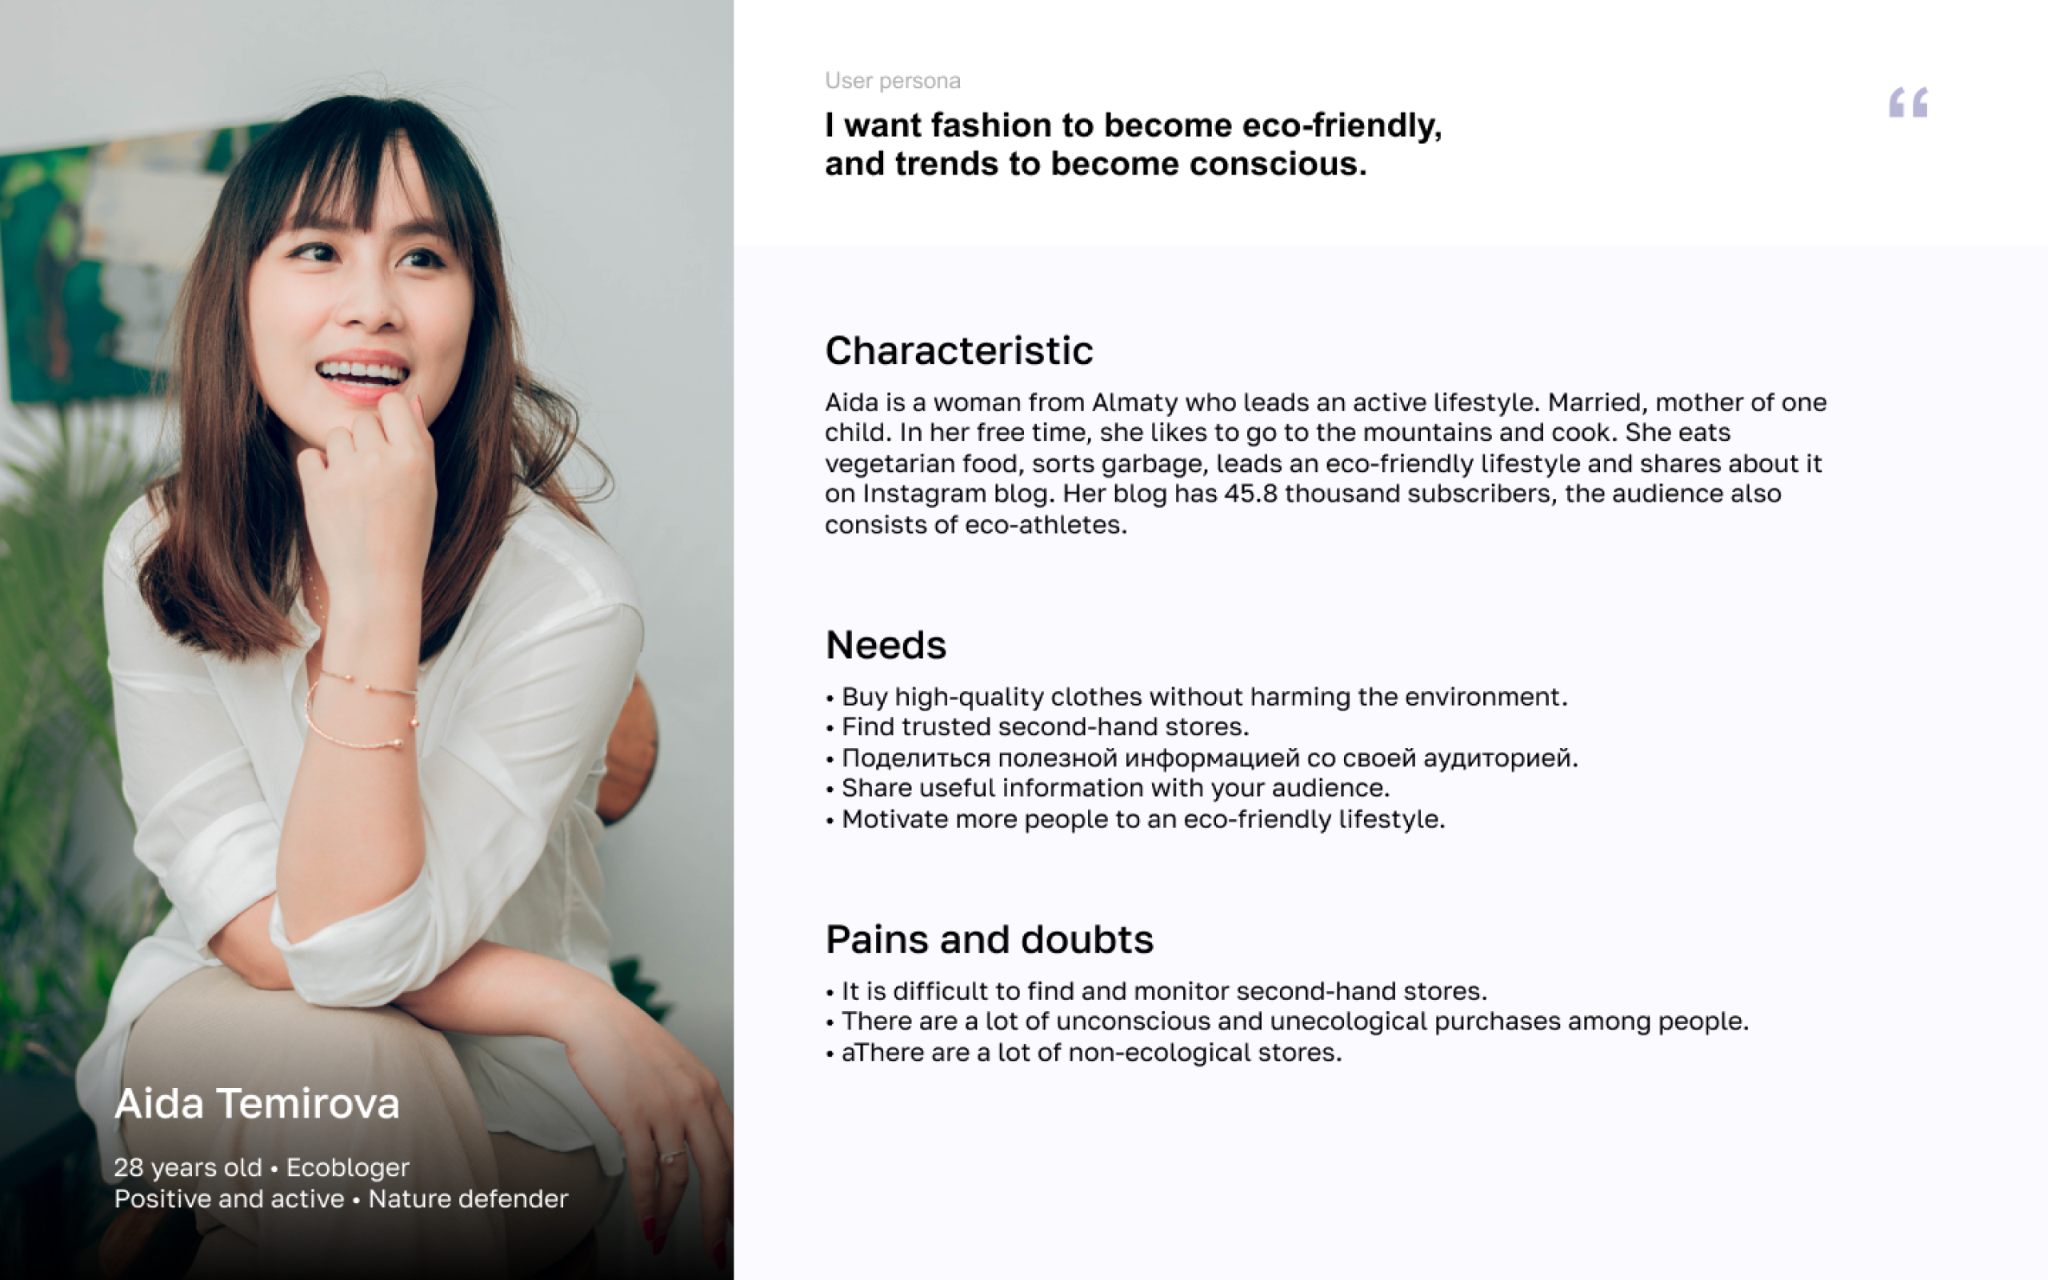
\includegraphics[scale=0.22]{figures/image001.png}
    \caption{user personas}
    \label{fig:image001}
\end{figure}
\begin{figure}[t!]
    \centering
    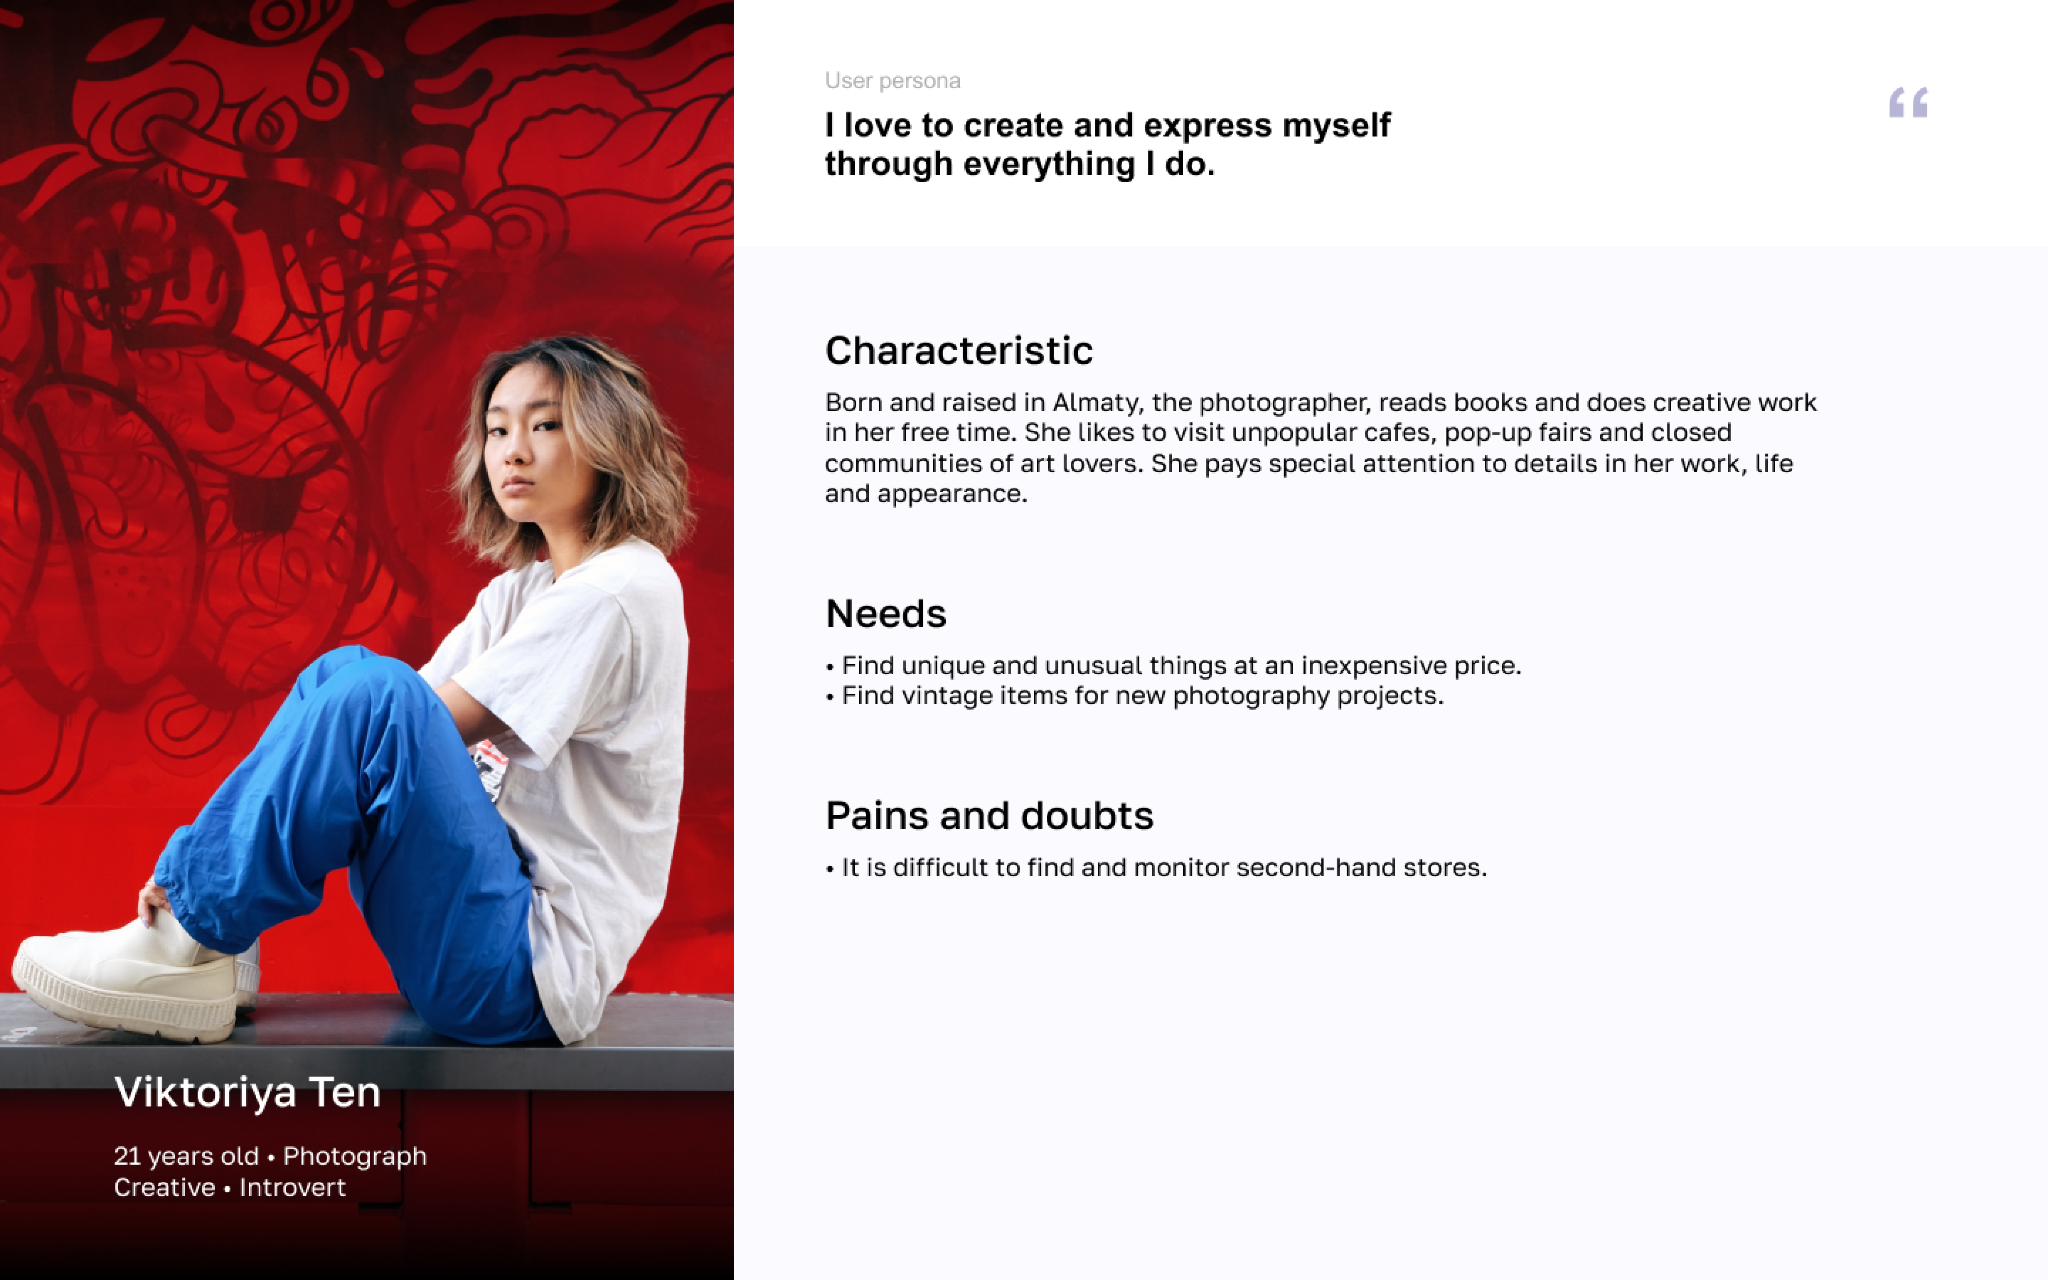
\includegraphics[scale=0.22]{figures/image003.png}
    \caption{user personas}
    \label{fig:image003}
\end{figure}

After understanding what aspects should be considered, we moved to the next step: Information Architecture. It’s a part of the UX process, where the hierarchy, navigation and structure of the visual part of the website are described. The scheme was constructed on the tool Miro. Design was separated for two roles: customer and shop owner.
Website structure for customer consists of: 

- Main page (main banner, main categories of products, auction of the day, products with sale, shops)

- Catalog (categories and subcategories, and clothes itself)

- Auctions (clothes on the auction)

- Shops

- Profile (personal information and orders journal)
Authorization\\

While for the shop owner:

- Authorization

- Dashboard (analytics)

- Catalog (Add, delete and edit products)

- Orders

- Shop (Editing information about shop)

The next stage was Designing Wireframes, which started from drawing simple prototypes abstractly showing location of each element and finishing with high fidelity wireframes grouped into flows(Our full design in Appendix \ref{app:A}). Figma was the most convenient tool for implementing this task, because it gives opportunity to make work more effective and consistent. (See Figure \ref{fig:image005},\ref{fig:image007}).

\begin{figure}[h]
    \centering
    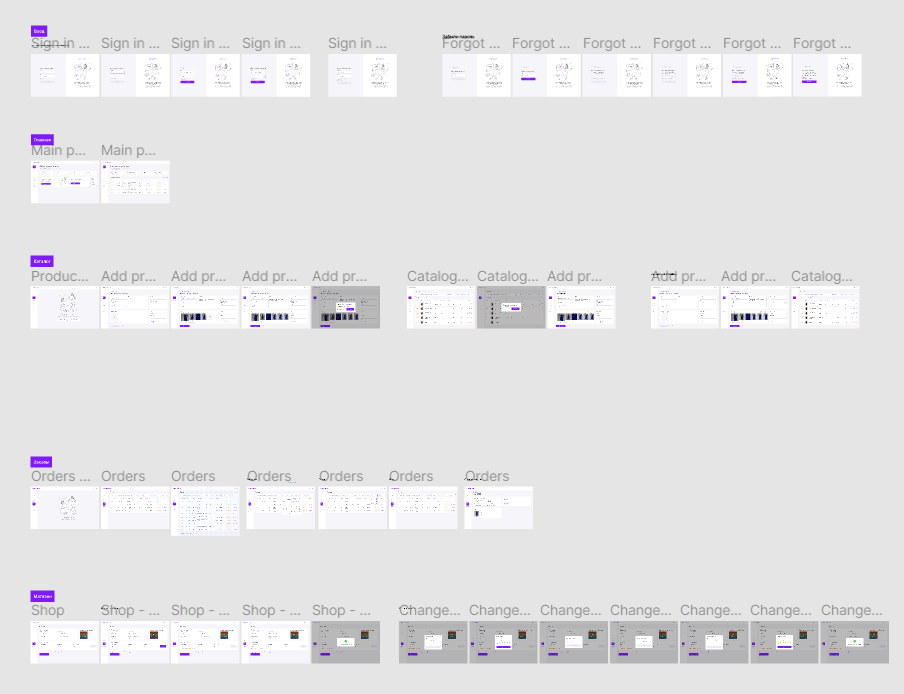
\includegraphics[scale=0.53]{figures/image005.png}
    \caption{Wireframes for shop owner}
    \label{fig:image005}
\end{figure}
\begin{figure}[pt!]
    \centering
    
\includegraphics[scale=0.33]{figures/image007.png}
    \caption{Client main page}
    \label{fig:image007}
\end{figure}
\clearpage
%Monkey is a beast that can jump. See Appendix \ref{app:B}.
\section{Project database}
There are many dbms (database management systems) to raise the database but our choice was
postgres\cite{greenpeace} because of its great advantages. (See Figure \ref{fig:database}).
\begin{figure}[ht!]
    \centering
    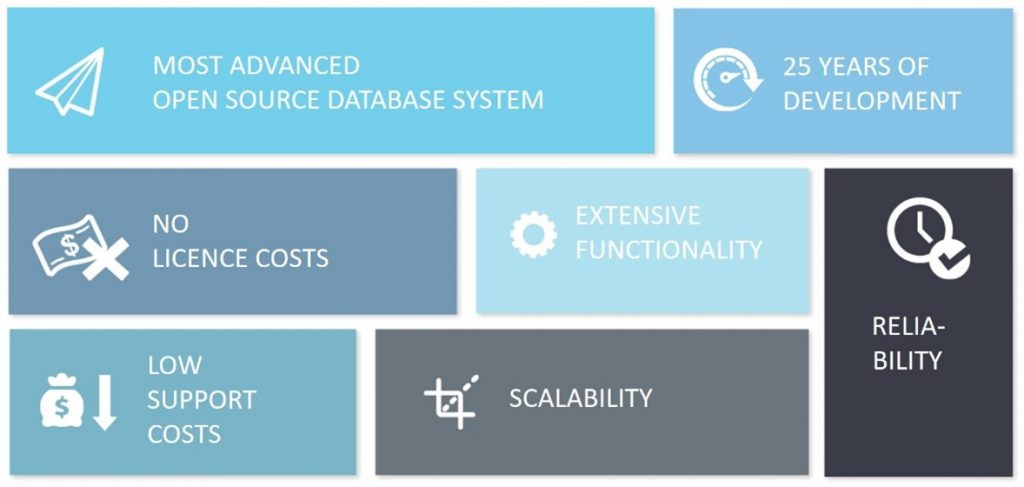
\includegraphics[scale=0.5]{figures/database.jpg}
    \caption{Advantages of postgres}
    \label{fig:database}
\end{figure}

However not all the features are used in our project, it is still the most comfortable dbms
and for more convenient data management, it was decided to make it remote, due to free
service heroku.

Although postgres is nice place to save data\cite{postgre}, in our project there is an auction
functionality and using just simple dbms would not be enough to meet the response speed
requirements. Therefore we used redis rdbms. Since no/sql languages   have an advantage over
just sql languages   for example data processing speed, scalability, distributed systems

Also to run our web site on a server we used ngrok for its simplicity and convenience
As a server we used Raspberry Pi because of its low cost, processing power, linux support, many
interfaces like HDMI, multiple USB, Ethernet, onboard Wi-Fi and so on.
\clearpage
\section{Back-end implementation}
In our project, we used the golang programming language for the backend part.Since, golang was created in order to be convenient to use and at the same time be very effective\cite{golang}. We also used redis to store the jwt token and the refresh token, as well as to store the prices of the goods for the auction. 

You can see the structure of our project. (See Figure \ref{fig:backend1}).
\begin{figure}[ht!]
    \centering
    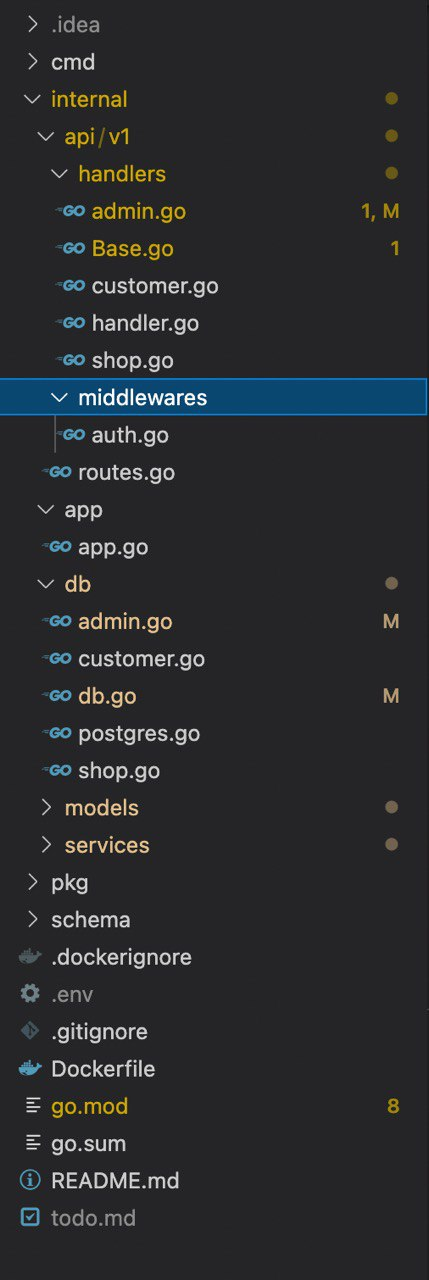
\includegraphics[scale=0.7]{figures/backend1.jpg}
    \caption{Structure of the project}
    \label{fig:backend1}
\end{figure}

We used a clean architecture, it makes the system easy to learn, simplifies development, deployment on the server, as well as maintenance of the software system. And most importantly, it gives flexibility and the opportunity to continue to have as many options as possible. Handlers provide communication with internal and external layers. (See Figure \ref{fig:backend2}). At the service level, we implement business rules, or rather, all cases of using the system. To do this, we use entities from the model level. The db folder serves as an external layer, it consists of a database and its details In the models folder, we have entities that are defined by business rules and that represent a set of data structures.
\begin{figure}[ht!]
    \centering
    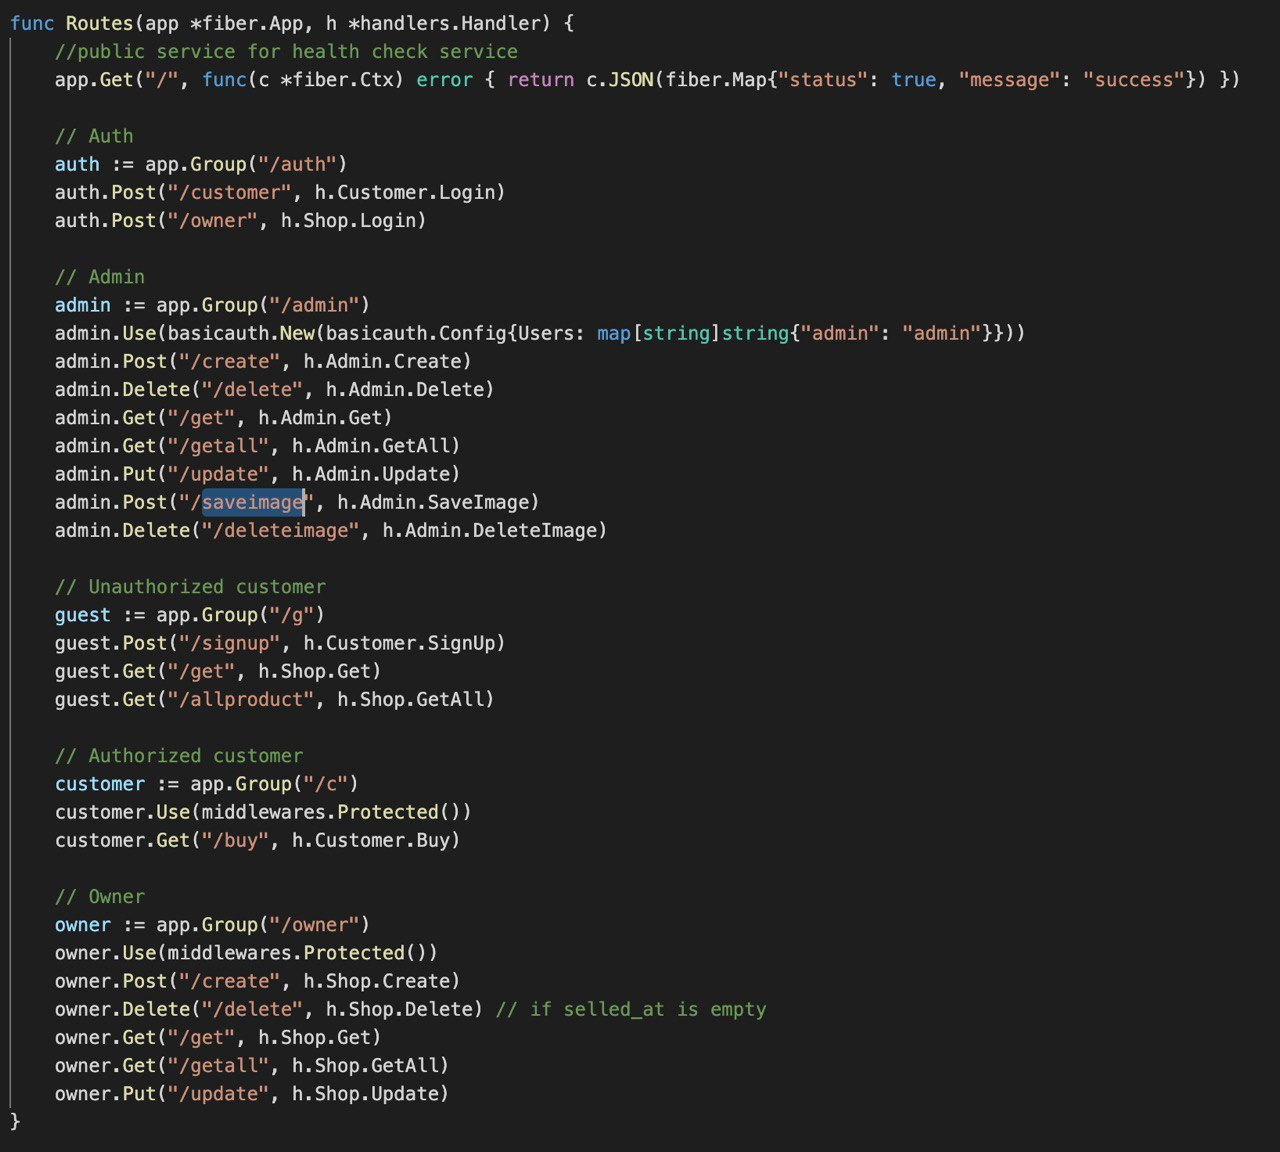
\includegraphics[scale=0.7]{figures/backend2.jpg}
    \caption{Handlers}
    \label{fig:backend2}
\end{figure}
\clearpage

\section{Front-end implementation}
This project's user section is for anyone who wants to buy old stuff. Ordinary users do not have access to the administrative section. We have numerous pages in the user section that differ in terms of information and functions. The main page of our site consists of search functions, as well as various information.(See in Figure \ref{fig:front-end})
\begin{figure}[h!]
    \centering
    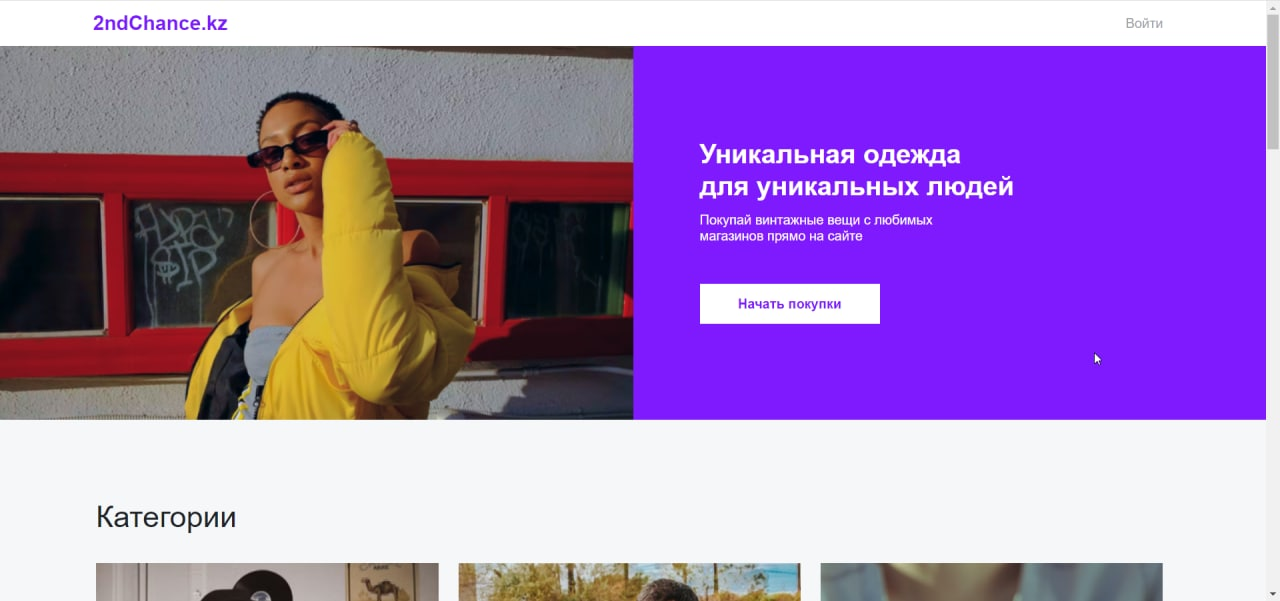
\includegraphics[scale=0.6]{figures/front-end.jpg}
    \caption{Main-page}
    \label{fig:front-end}
\end{figure}

Such as: categories, discounts of the day, auctions, shops. There are also pages such as a catalog, product details and a payment page. Several libraries were used in the creation of this site, and one of them is the most up-to-date bootstrap library. The entire front-end site was written in react js.React - JavaScript library, which helps to build UI part. Since, it's flexible and has great performance\cite{react}.

The front-end of our website consists of two parts, admin and client. The admin part is for second hand stores that display their products. This part helps sellers to lay out their goods. And the second is the client part, this is for users and buyers. So, the whole design was written in react.js, so it is connected to the golang backend.

    \chapter{Conclusion}\label{ch:concl}
Everything is great, but there is a space for future work.
    
    \appendix
    \chapter{Design part}\label{app:A}

\begin{figure}[h!]
    \centering
    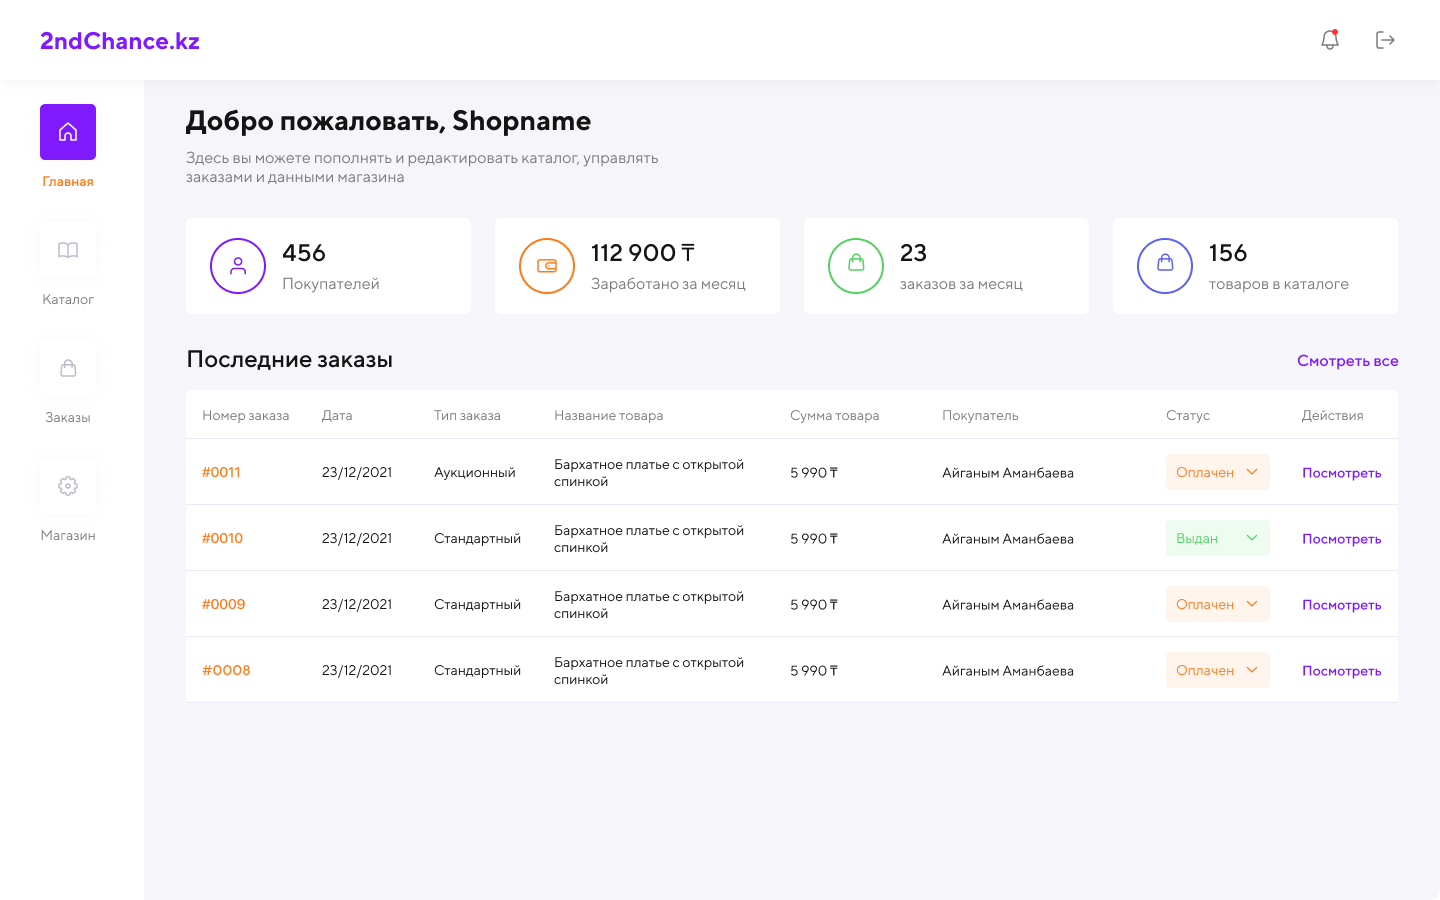
\includegraphics[scale=0.3]{figures/Main page.png}
    \caption{Main page}
    \label{fig:main-page}
\end{figure}

\begin{figure}[h!]
    \centering
    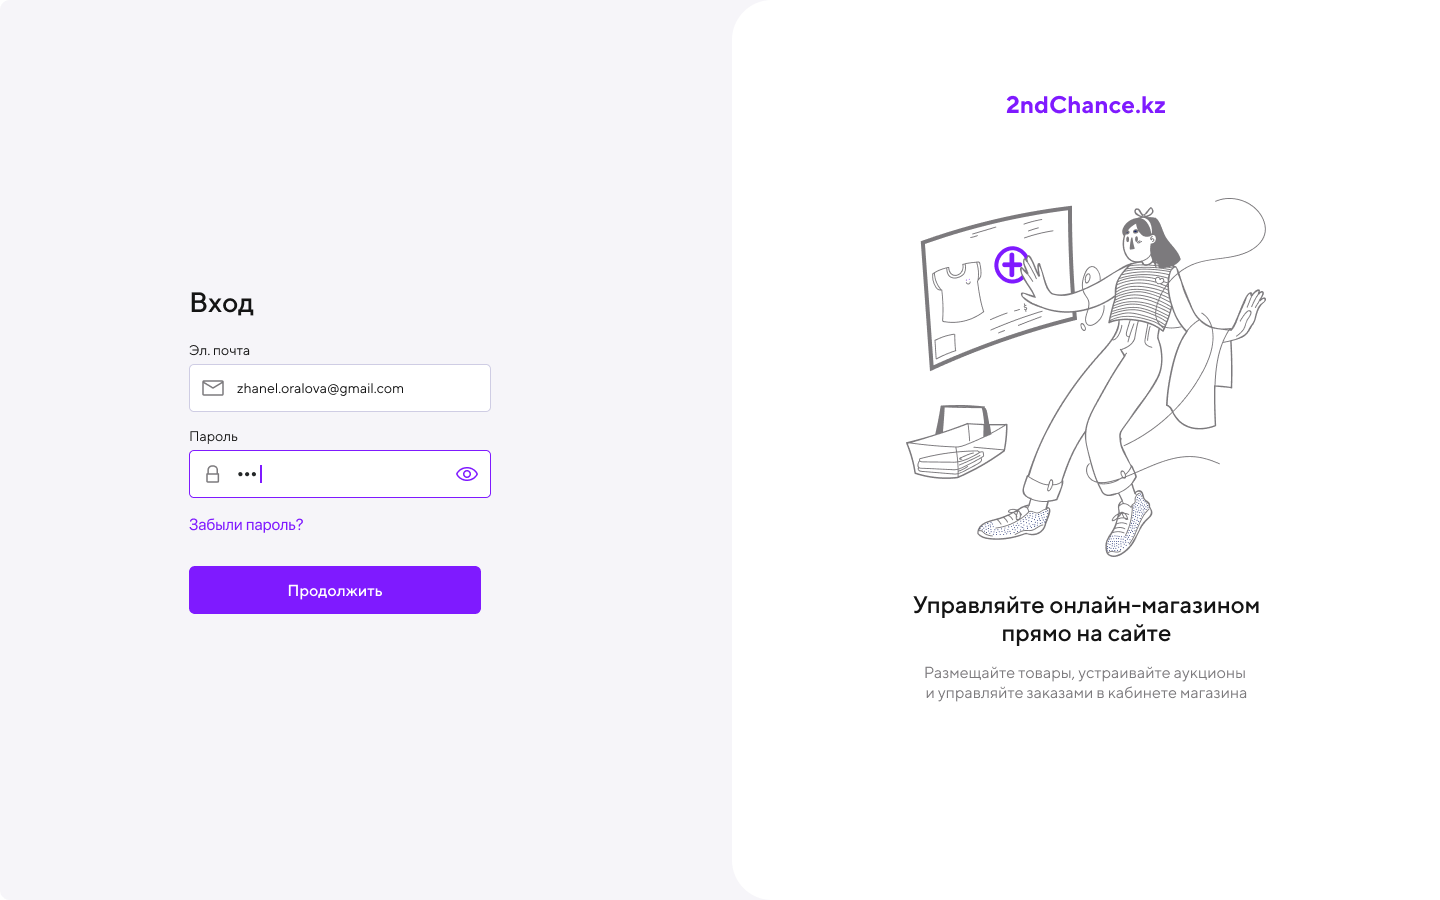
\includegraphics[scale=0.3]{figures/Sign in password active.png}
    \caption{Sign in page}
    \label{fig:sign-in}
\end{figure}
\begin{figure}[h!]
    \centering
    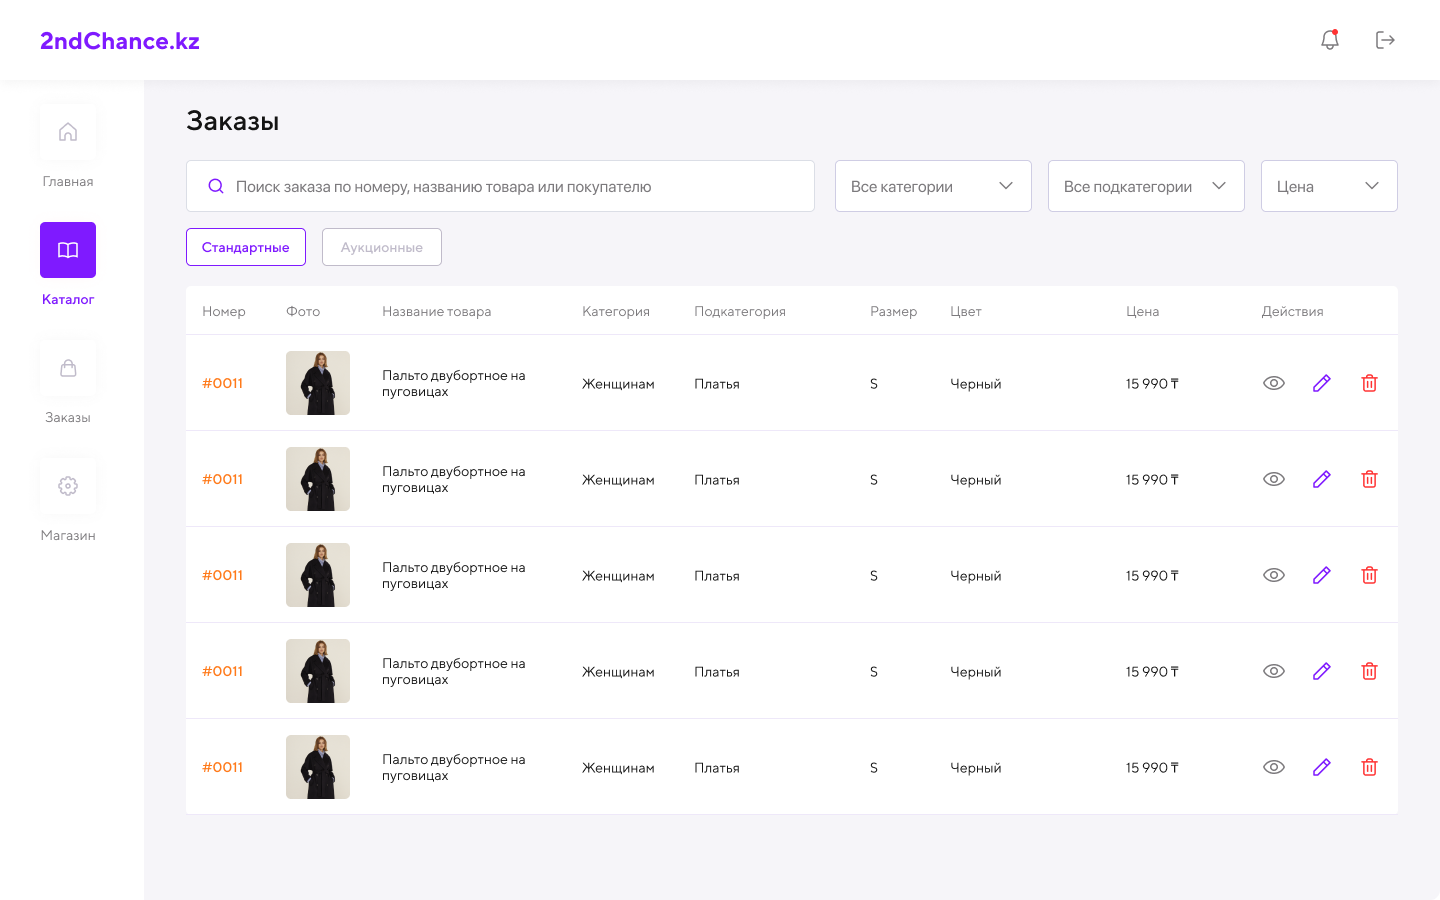
\includegraphics[scale=0.3]{figures/Catalogue Filled.png}
    \caption{Catalog page}
    \label{fig:catalogue page}
\end{figure}

\begin{figure}[h!]
    \centering
    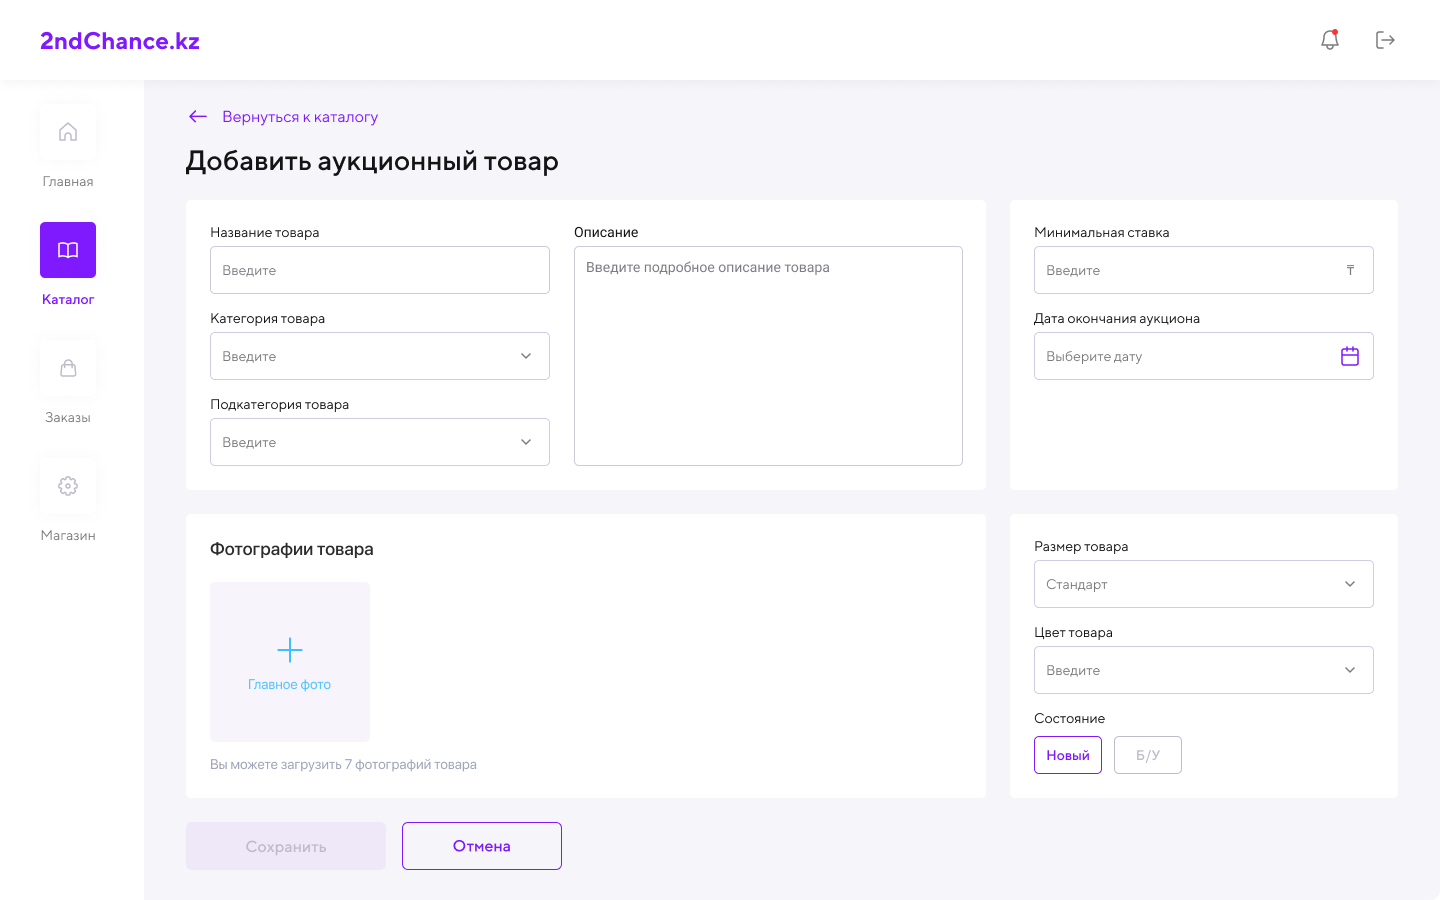
\includegraphics[scale=0.3]{figures/Add product.png}
    \caption{Add product page}
    \label{fig:add product}
\end{figure}
\begin{figure}[h!]
    \centering
    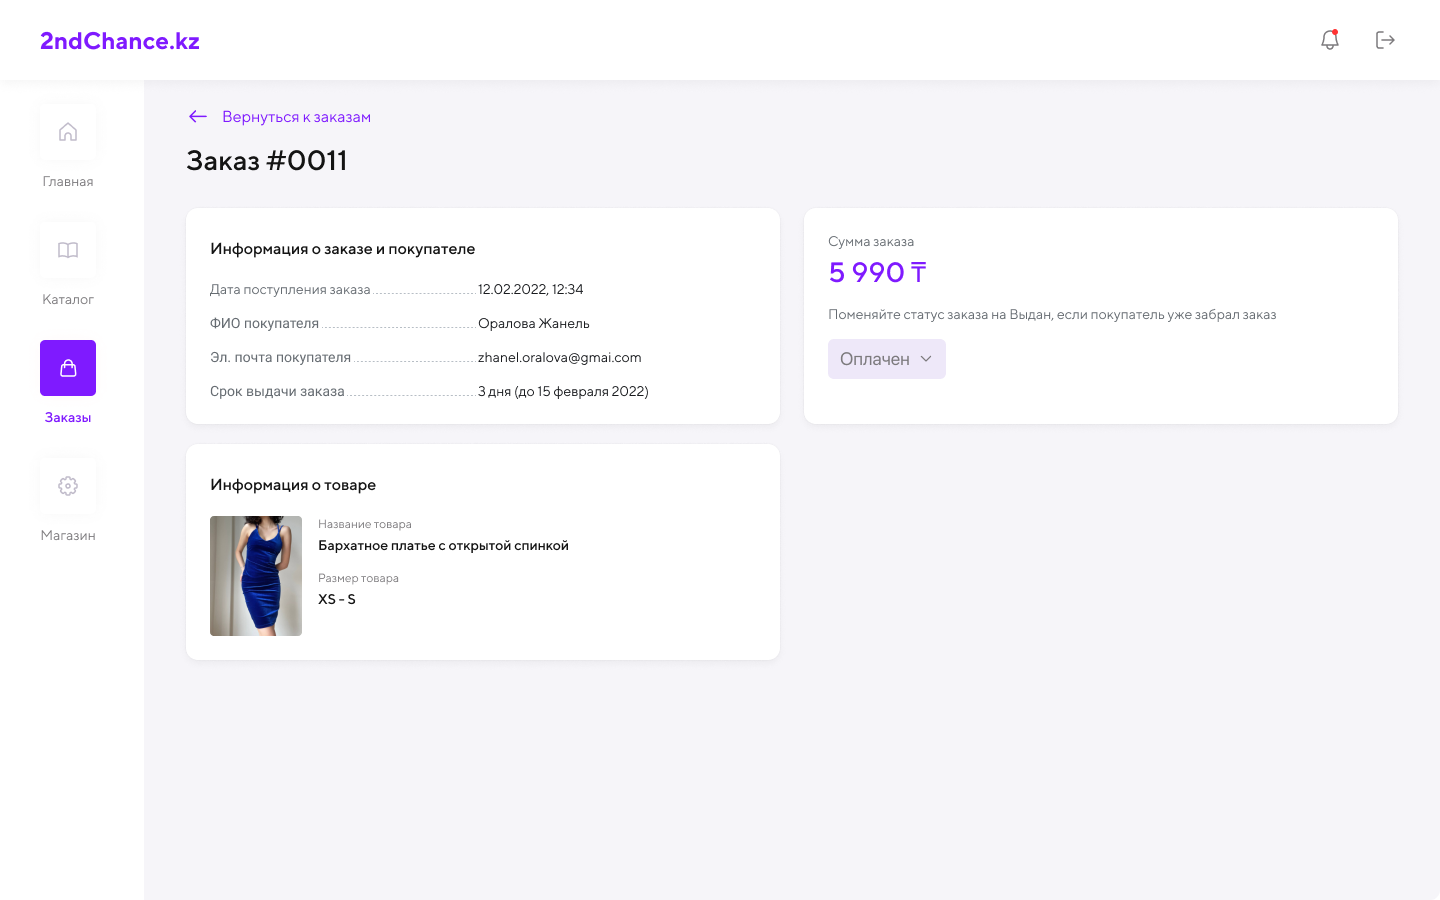
\includegraphics[scale=0.3]{figures/Orders.png}
    \caption{Orders page}
    \label{fig:orders page}
\end{figure}
\begin{figure}[h!]
    \centering
    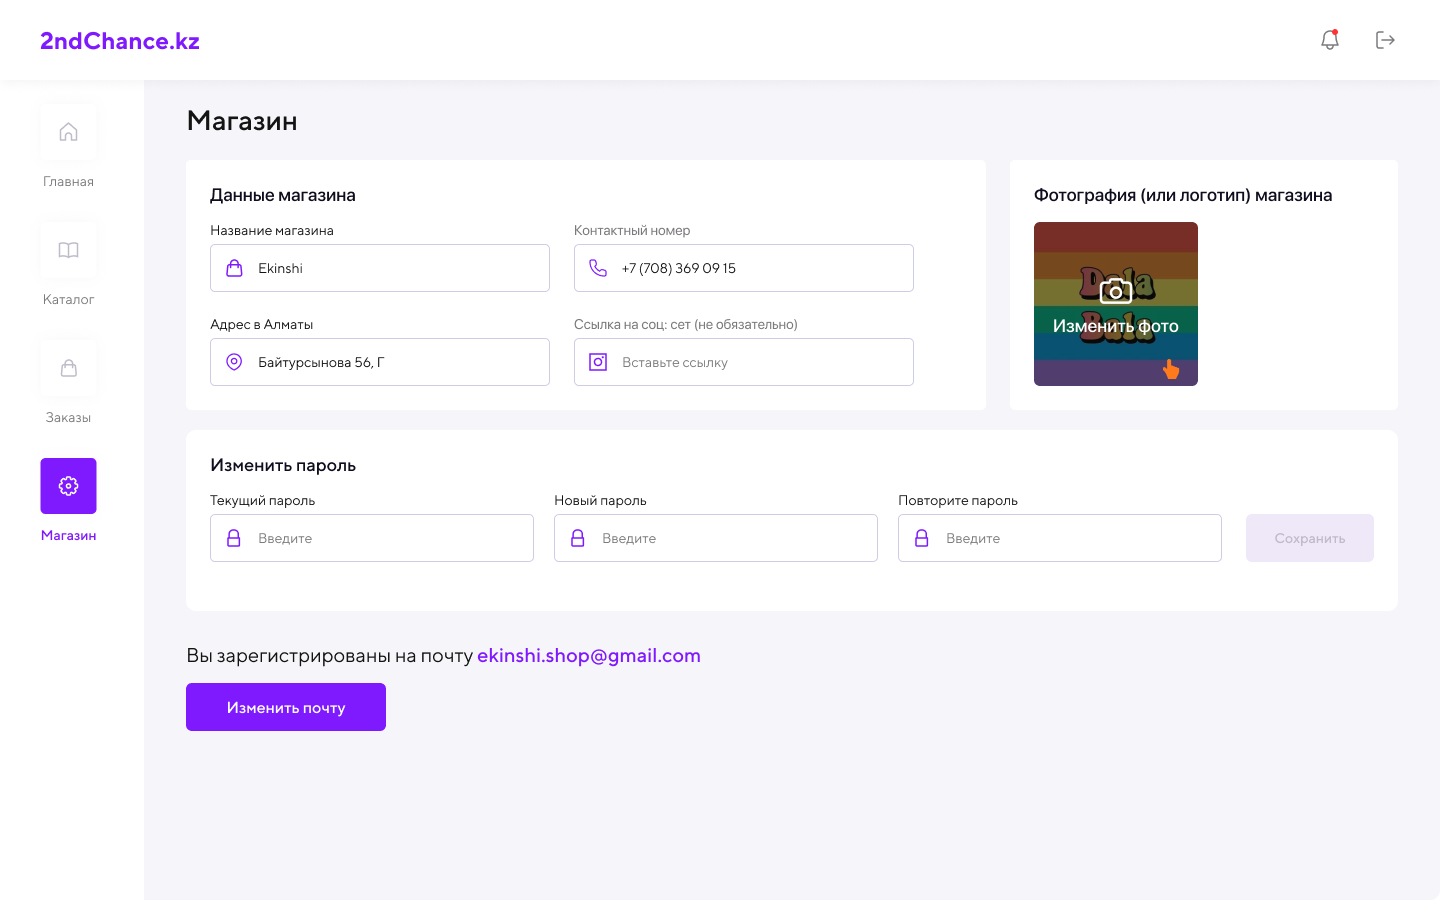
\includegraphics[scale=0.3]{figures/Shop.png}
    \caption{Shop page}
    \label{fig:shop page}
\end{figure}


   
    
    
    
    
    \printbibliography[heading=bibintoc,title={References}]
\end{document}
